\section{O estilo dos slides}

Os slides devem apresentar uma identidade conjunta. Para isso devem ser usados estilos apropriados, que estão disponíveis nas ferramentas de criação, ou se criar um estilo novo. A Figura \ref{fig:tres} mostra três slides diferentes em estilo e que mantêm uma identidade conjunta por meio de cores, fontes e rodapés.

Esse estilo deve possuir vários tipos de slides. A aula deve usar mais de um desses tipos, tanto para cumprir papéis posicionais, como o título, quanto para não ficar monótona. Os tipos principais são:
\begin{itemize}
    \item título;
    \item o título de seção;
    \item o slide de uma coluna, o mais comum;
    \item o slide de duas colunas;
    \item o slide de duas colunas com títulos, e
    \item o slide só com título, usado para figuras.
\end{itemize}


A Figura \ref{fig:tiposbasicosdopp}, copiada do \textit{Power Point} mostra esses seis tipos principais e mais alguns disponíveis para uma apresentação em branco, como o slide branco, e dois modelos com legenda.

\begin{figure}[htb]
    \centering
    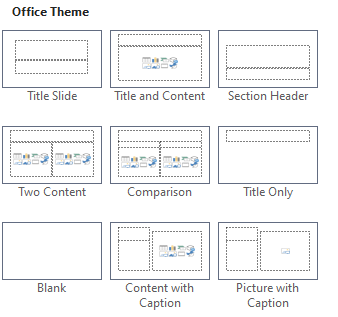
\includegraphics[width=0.5\linewidth]{imagens/tiposbasicosdopp}
    \caption{Slides básicos disponíveis no Power Point}
    \label{fig:tiposbasicosdopp}
\end{figure}

Cada tipo de uso, como apresentação, aula, defesas ou exames, tem um tipo de slide mais adequado, de acordo com a necessidade de chamar atenção, e o grau de formalidade.

Em qualquer tipo de uso, porém, existem alguns objetos que devem aparecer nos slides, como a numeração e a identificação do autor e da instituição.

Os slides \textbf{devem ser numerados} e conter em cada slide o número total de slides, possivelmente no formato ``slide/total'', como em ``4/40''. Os números não podem ser pequenos, e eu favoreço números grandes, para que fique bem claro e possam, mesmo a distância, serem usados como referência. Esse número fica normalmente no pé (\textit{footer}) do cabeçalho.

Também é importante ter a identificação do autor. Normalmente ela inclui um e-mail ou um site.

Além disso, é interessante que, para a maioria dos usos, o estilo do slide esteja diretamente associado a uma instituição. Isso pode ser feito por meio da colocação do logo da instituição em uma posição clara.

No Power Point existem, por \textit{default}, três espaços no rodapé do slide (\textit{footer}). Um é reservado para o número. Os outros dois são possivelmente livres, sendo que um  sempre devemos usar identificar o autor. O terceiro espaço pode ser usado para o título da apresentação, o título do curso, o título do evento ou outra informação similar que se quer ressaltar.

A Figura \ref{fig:coppe} mostra um slide com todos esses elementos: o logo do PESC, o nome e e-mail do autor, o nome do curso, o número do slide em uma fonte grande e o número total de slides em uma fonte menor.



Devemos usar fontes ``limpas'', não rebuscadas, e \textbf{sem-serifa}\footnote{Serifas são as pontinhas que existem em algumas fontes. Elas estão bem visíveis no S da palavra ``slides'' desta seção.}, como Arial ou Calibri, e \textbf{corpos grandes}, 32 pts, por exemplo. Os slides das Figuras \ref{fig:coppe} e \ref{fig:teximag} seguem essa regra. Já o slide da figura \ref{fig:formulas} usa um tamanho menor para o corpo das fórmulas. Lembre que a banca, ao invés dos alunos, é mais velha e pode ter dificuldades de visão.





\subsection{Usando os logos corretos}

É importantíssimo usar os logos corretos das instituições. Para isso procure os logos originais e os manuais de marca.

A lista de logos que eu uso é:
\begin{itemize}
    \item UFRJ: \url{https://ufrj.br/comunicacao/manuais-e-modelos/marca-da-ufrj/}
    \item COPPE: \url{https://www.coppe.ufrj.br/pt-br/a-coppe/uso-da-marca}
    \item PESC:  \url{https://www.cos.ufrj.br/index.php/pt-BR/logo-pesc}
    \item IM: não fornece o logotipo na página, porém é possível copiar. A história da marca principal está em \url{https://sites.google.com/matematica.ufrj.br/mapcabral/outros/hist%C3%B3ria-do-logotipo-do-im}
    \item DCC: não fornece o logotipo na págica, mas, de qualquer maneira, será transformado no IC, com novo logotipo
    \item POLI: \url{http://www.poli.ufrj.br/marcadapolitecnica.php}
    \item LUDES: \url{https://github.com/LUDES-PESC/Generico/tree/master/Logo%20Novo%20Vers%C3%B5es}
    \item LINE: \url{https://github.com/LINE-PESC/Generico/tree/master/Logomarca%20LINE}
\end{itemize}

No GitHub deste documento estão disponíveis algumas sugestões de slides.


\subsection{Nomeando os slides}

Todo slide deve ter um \textbf{título único}. Esse espaço já vem reservado nos estilos de \textit{Power Point}.

Algumas pessoas, erroneamente, usam um título de seção que se repete nessa posição e colocam o que seria o título do slide como uma caixa-de-texto, ou como primeiro item da lista de itens do slide. Essa prática faz com que a audiência se perca em relação a onde o apresentador está. O nome e o número do slides servem não só para identificá-los, mas também como posicionamento na sequência.

É possível criar um slide com o nome da seção, mas ele deve ser menor que o nome do slide. Usando o \texttt{beamer}, o formato de slides do \LaTeX, é possível colocar no topo do slide uma mini-agenda, onde o nome da seção tem uma ênfase. A Figura \ref{fig:meio} mostra um slide que tem todas as seções identificadas em seu cabeçalho, sendo que a seção atual está com ênfase.





\subsection{Variando e inventando}


É importante variar o estilo do slide. Isso é bem fácil no \textit{Power Point}, porém é mais difícil no \texttt{beamer}, por exemplo. A Figura \ref{fig:man} mostra um slide bem diferente do que os apresentados normalmente, mas ainda em um formato ``retangular''. Use os formatos para tirar a monotonia da aula. Use também animações nos slides, mas cuidado com as transições entre os slides, que devem ser usadas muito parcimoniosamente, porque quebram a atenção.

\begin{figure}[htb]
    \centering
    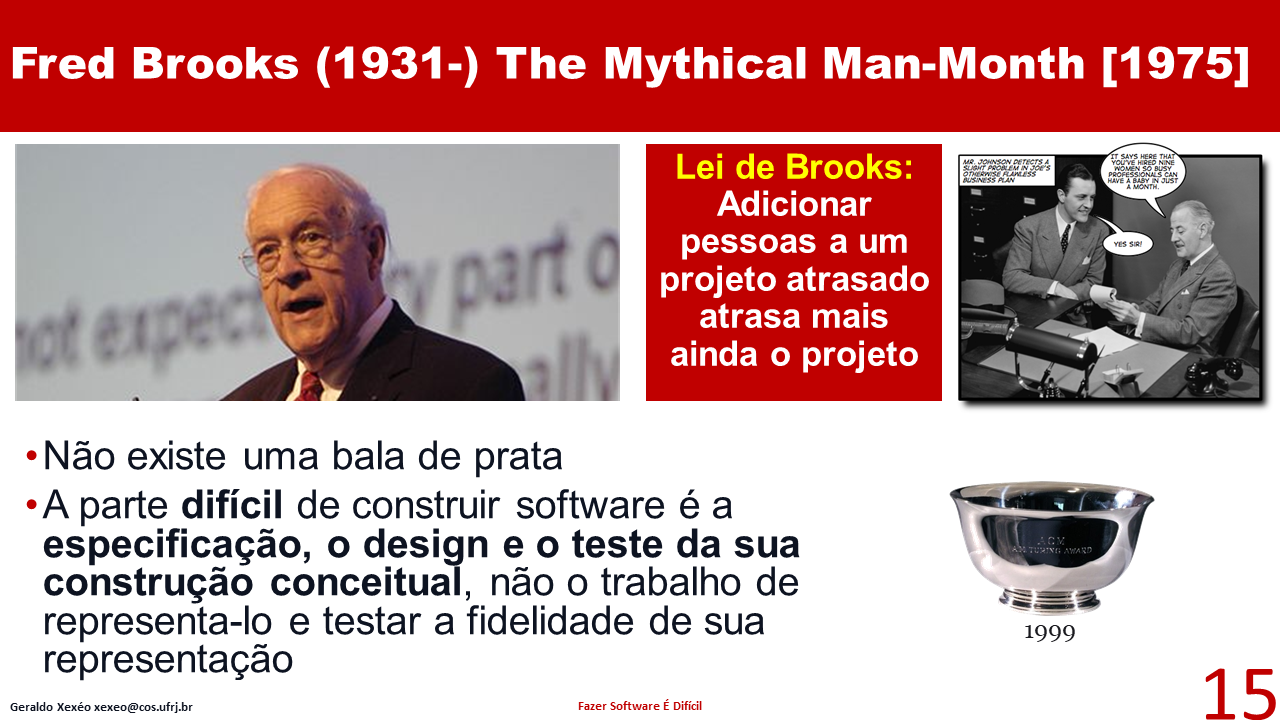
\includegraphics[width=\tam\linewidth]{imagens/manmonth.png}
    \caption{Um slide com um formato diferente}
    \label{fig:man}
\end{figure}

Os slides não devem ser exagerados, nem em texto, nem em decoração, porém um ou outro slide pode ser mais divertido, ou mais pesado em texto.


Em um slide com fórmulas, como o da Figura \ref{fig:formulas}, elas devem aparecer uma a uma se estiverem sendo calculadas. Se for apenas um comentário sobre a complexidade das fórmulas, que você deseje passar por cima em busca de uma explicação mais fácil, elas podem aparecer todas de uma vez.

\begin{figure}[hbt]
    \centering
    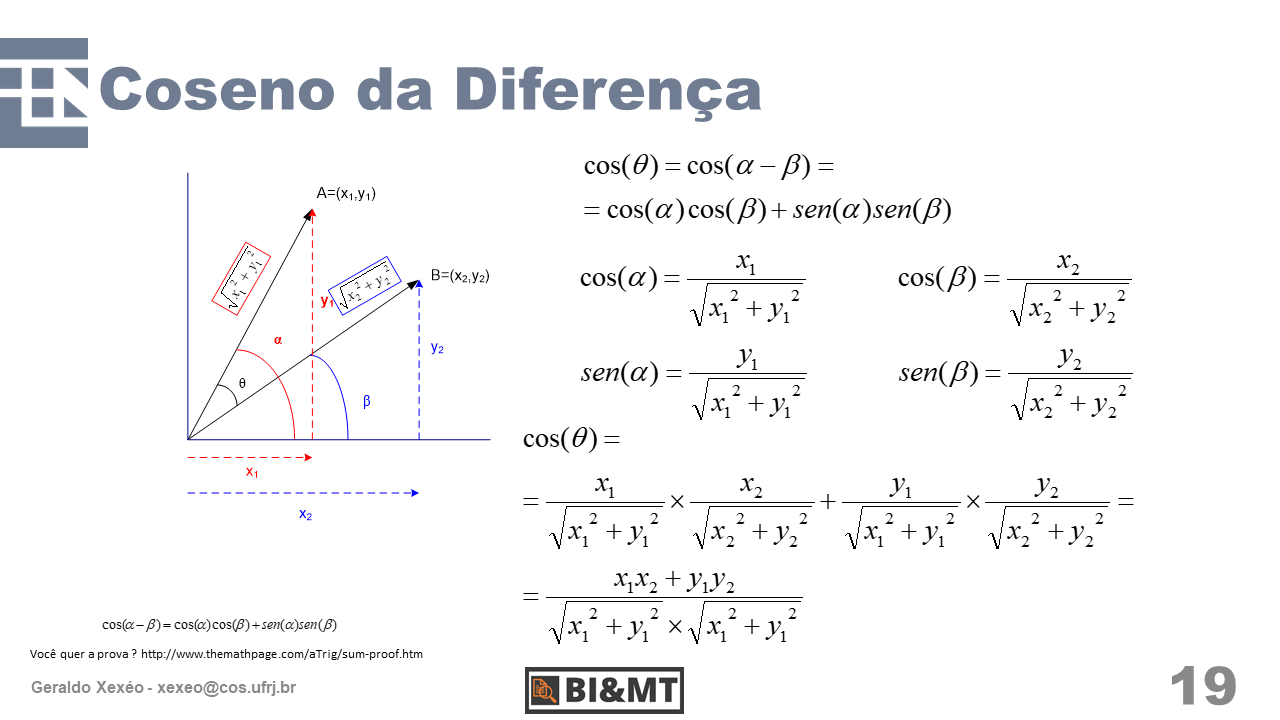
\includegraphics[width=\tam\linewidth]{imagens/desenhoeformulas.png}
    \caption{Desenho e fórmulas em um slide, que possui o logo do laboratório ligado ao curso e um logo que foi criado para identificar o curso em 3 lugares: Moodle, Whatsapp e GitHub.}
    \label{fig:formulas}
\end{figure}



Slides ``divertidos'', como os que estão resumidos\footnote{Esses slides foram encontrados em     \url{https://unblast.com/funtastic-free-powerpoint-presentation-template-ppt/}
} na Figura \ref{fig:fun} vão criar uma carga cognitiva muito grande em uma apresentação e podem incomodar membros da banca. Já vi isso acontecer. Mas isso não quer dizer que não possam ser usados em um ou outro slide, como marcos de início de seção ou outra alternativa de menor impacto que usá-los em toda aula.

\begin{figure}[hbt]
    \centering
    
\includegraphics[width=\tam\linewidth]{imagens/funslide.jpg}
    \caption{Exemplos de slides divertidos.
        (Fonte: unblast.com) }
    \label{fig:fun}
\end{figure}

\subsection{Quebrando as regras}

É possível quebrar as regras algumas vezes para tirar a monotonia das aulas ou para deixar um ponto mais claro.

No slide da Figura \ref{fig:magica} fiz uma brincadeira com a turma, para chamar atenção em meio a uma aula expositiva onde não havia atividades. Para auxiliar a quebrar o ritmo escolhi, apenas nesse slide da aula, usar uma fonte totalmente diferente, que inclusive dificulta  a leitura, mas que tenta simular uma fonte mágica.

\begin{figure}[tbh]
    \centering
    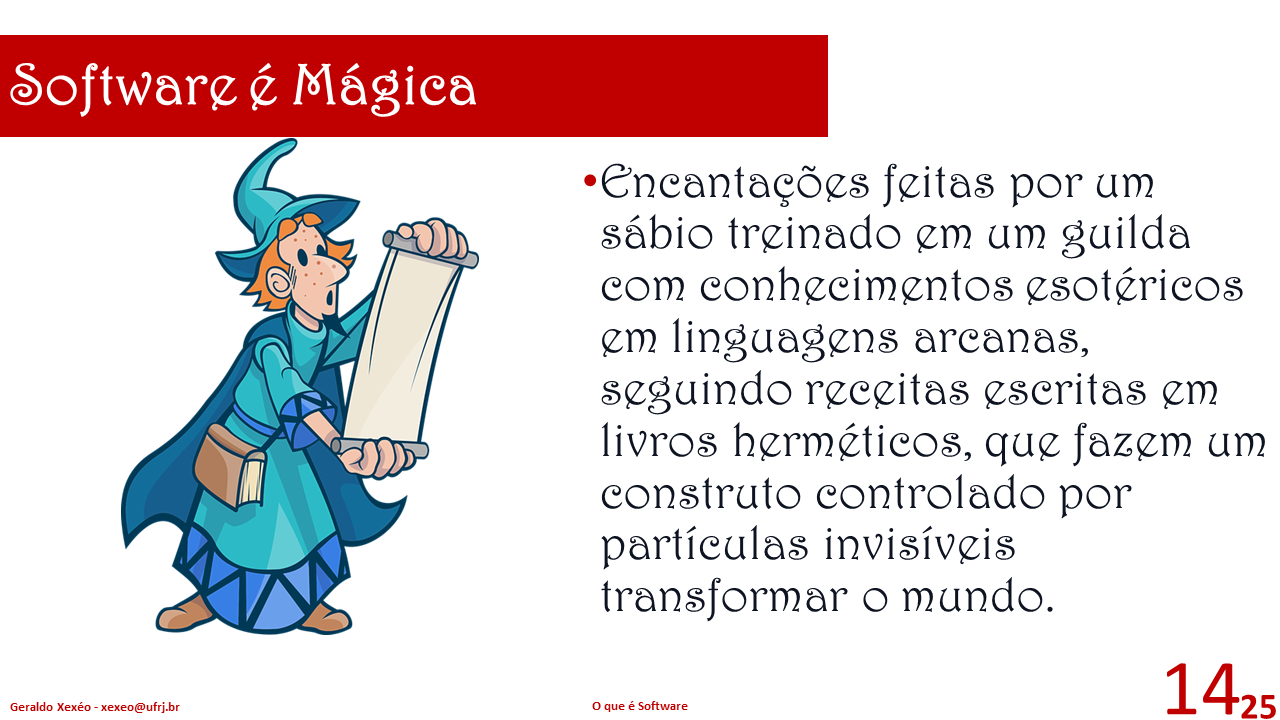
\includegraphics[width=0.7\linewidth]{imagens/magica}
    \caption{Slide feito para ``acordar'' e motivar a turma em uma aula que explica o que é software.}
    \label{fig:magica}
\end{figure}

Já o slide da Figura \ref{fig:ponte} usa a técnica da ``figura inspiradora'', que eu não considero correta para toda uma aula, e também não tem título. Mas ele aparece logo depois de um slide comum que acaba com a sentença ``Um projeto é uma ponte do estado atual para um futuro melhor''. Eu uso o slide para explicar melhor o conceito de por que fazemos projeto, mas ele está lá para motivar e mudar um pouco o tom da aula, até aquele momento com slides de definição e instrução. Nesse momento o slide serve de cenário para os comentários, mas o slide anterior garante que a ideia específica está registrada.

\begin{figure}[tbh]
    \centering
    
\includegraphics[width=0.7\linewidth]{imagens/ponte}
    \caption{Figura da ponte só aparece porque no slide anterior há a frase ``Um projeto é uma ponte do estado atual para um futuro melhor''}
    \label{fig:ponte}
\end{figure}



\subsection{Slide de contato}

Como adicional, toda apresentação deve possuir um slide final que indica um contato. Hoje, todas as minhas aulas terminam com o slide da Figura \ref{fig:fim}. Isso pode ser usado sempre para falar algo como ``quem quiser me contatar para tirar dúvidas...''.

\begin{figure}[h]
    \centering
    
\includegraphics[width=\tam\linewidth]{imagens/fim.png}
    \caption{Um slide de contato.}
    \label{fig:fim}
\end{figure}



